
\begin{figure}
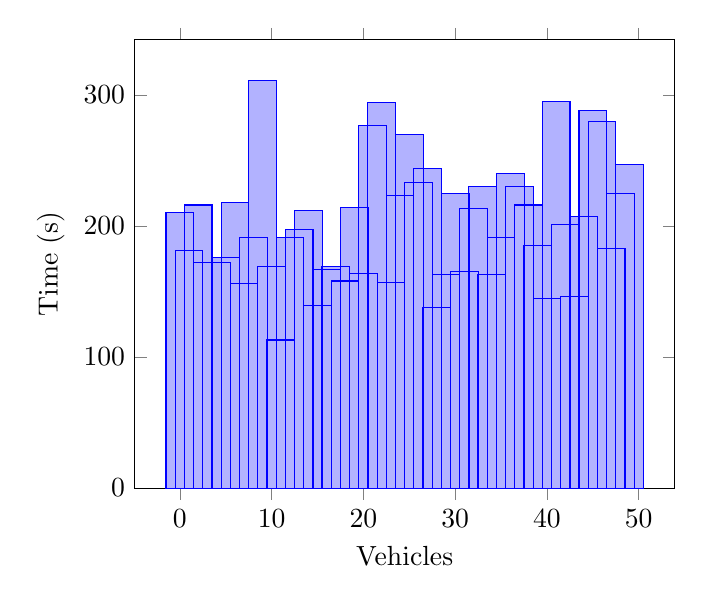
\begin{tikzpicture}
\begin{axis}[
legend style={anchor=west},
xlabel=Vehicles,
ylabel=Time (s),
ymin=0,
ybar,
]
\addplot coordinates {
(0, 210)
(1, 181)
(2, 216)
(3, 172)
(4, 172)
(5, 176)
(6, 218)
(7, 156)
(8, 191)
(9, 311)
(10, 169)
(11, 113)
(12, 191)
(13, 197)
(14, 212)
(15, 139)
(16, 167)
(17, 169)
(18, 158)
(19, 214)
(20, 164)
(21, 277)
(22, 294)
(23, 157)
(24, 223)
(25, 270)
(26, 233)
(27, 244)
(28, 138)
(29, 163)
(30, 225)
(31, 165)
(32, 213)
(33, 230)
(34, 163)
(35, 191)
(36, 240)
(37, 230)
(38, 216)
(39, 185)
(40, 145)
(41, 295)
(42, 201)
(43, 146)
(44, 207)
(45, 288)
(46, 280)
(47, 183)
(48, 225)
(49, 247)
};

\end{axis}
\end{tikzpicture}
\label{tik:100:91}
\caption{100 percent diving with GSC on route $91$}
\end{figure}
